\documentclass[tikz]{standalone}
\usepackage{pgfplots}
\pgfplotsset{compat=1.15}
\usepackage{mathrsfs}
\usetikzlibrary{arrows,calc}
\usepackage{tkz-euclide}

\pagestyle{empty}

\definecolor{AngleClr}{rgb}{0,0.39215686274509803,0}
\definecolor{ShapeClr}{rgb}{0.6,0.2,0}

\begin{document}

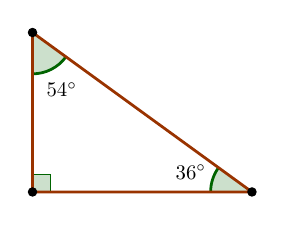
\begin{tikzpicture}[scale=.75]
\tkzSetUpLine[line width=1pt,color=black]
\tkzSetUpPoint[fill=black]

\tkzDefPoints{0/0/A,0/2.7/B,3.7162/0/C}


\tkzFillPolygon[fill=white](A,B,C)

\tkzFillAngles[size=.85,fill=AngleClr,size=0.7,fill opacity=0.2](A,B,C B,C,A)
\tkzMarkAngles[size=.85,line width=1pt,size=0.7,color=AngleClr](A,B,C B,C,A)

\tkzLabelAngle[pos=1.45,scale=0.75](A,B,C){$54^\circ$}
\tkzLabelAngle[pos=1.45,scale=0.75](B,C,A){$36^\circ$}

\tkzMarkRightAngles[line width=0.5pt, size=.3,color=AngleClr,fill=AngleClr,fill opacity=0.2](C,A,B)

\tkzDrawPolygon[color=ShapeClr](A,B,C)
\tkzDrawPoints[size=3](A,B,C)



\end{tikzpicture}

\end{document}
